\documentclass[a4paper,11pt]{article} 
\usepackage{latexsym} 
\usepackage[MeX]{polski} 
\usepackage{indentfirst}
\usepackage{graphicx}
\usepackage[utf8]{inputenc}

\usepackage{fancyhdr}
\pagestyle{fancy}
\usepackage{lastpage}
\fancyfoot[C]{Page \thepage \hspace{1pt} of \pageref{LastPage}}

\graphicspath{ {images/} }
\author{} 
\title{
	\Huge Specyfikacja implementacyjna \\
	automat komórkowy\\
	\textbf{"The game of life"}
} 
\frenchspacing 
\begin{document}
  %Strona tytułowa 
	\maketitle 
	\newpage
	\tableofcontents 
	\newpage
	\section {Informacje ogólne}
		\subsection{Nazwa programu}
			Nazwa programu: \texttt{life\_game\_generator}
		\subsection{Język}
			Program został napisany w języku~C i~jest przystosowany do uruchomienia w~standardzie znajdującym się na serwerze ssh:~\textit{ssh.jimp.iem.pw.edu.pl}.
		\subsection{Uruchomienie programu}
			Program jest przeznaczony do~uruchomienia z~interfejsu tekstowego. Odpowiednie parametry przekazywane w linii poleceń pozwalają sterować programem i~uzyskać oczekiwane rezultaty. 
			\subsubsection{Wywołanie}
				\texttt{life\_game\_gen \textbf{[ścieżka generacji początkowej] [liczba generacji] [rodzaj sąsiedztwa] [nazwa katalogu wyjściowego]}}.
			\subsubsection{Przykładowe wywołanie} 				
				\texttt{life\_game\_gen~fgen.txt~10~-M~10gen}
				\newpage
\section{Diagram modułów} 
	\begin{figure}[h]
	  \centering
	  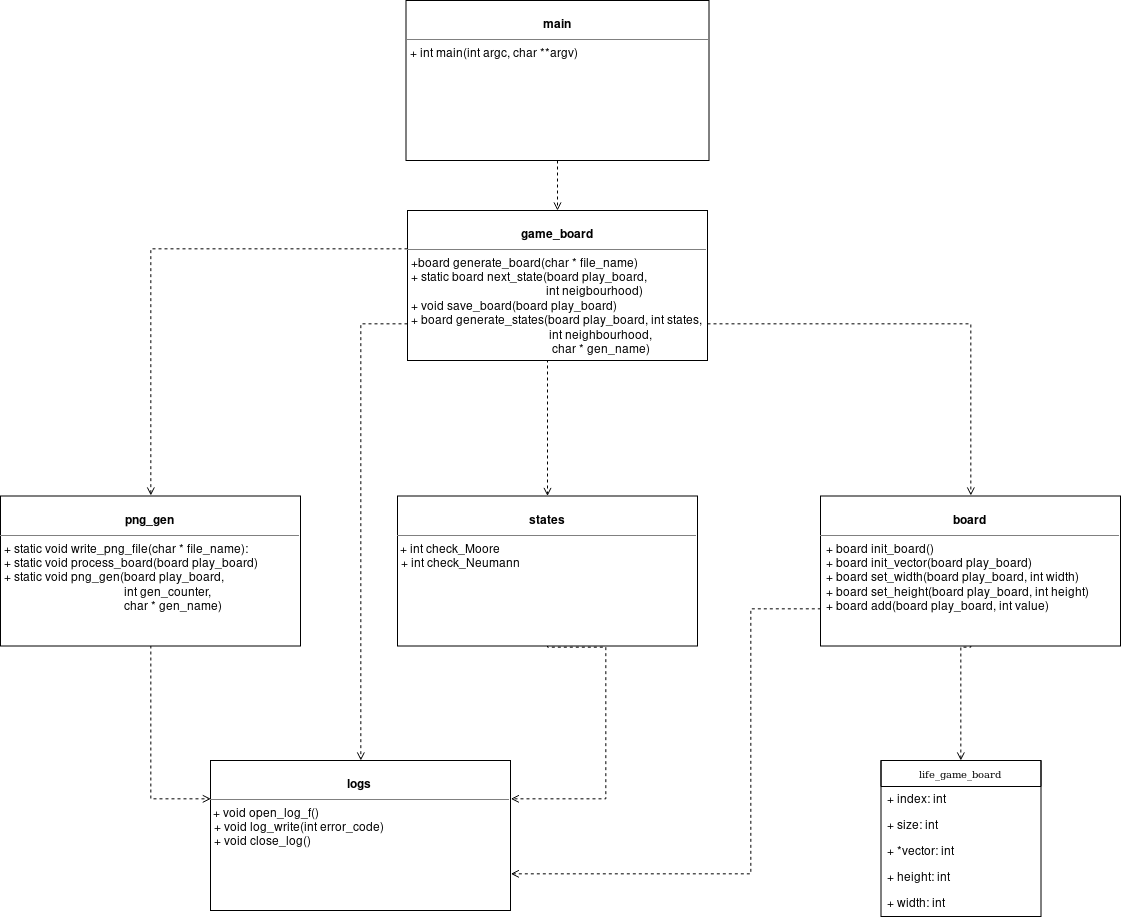
\includegraphics[scale=0.4]{diag.png}
	  \caption{Diagram modułów}
	  \label{fig:}
	\end{figure}
	%Diagram modułów(skierowanie strzałek, uzasadnienie)
	  \subsection{Relacje modułów}
	  	Moduł \texttt{main} zawiera funkcję sterującą, komunikuje~się on~bezpośrednio z~modułem \texttt{game\_board}, który jest odpowiedzialny za obsługę planszy i~przeprowadzanie kolejnych generacji. Moduł ten jest bezpośrednio związany z~modułem \texttt{board}, w którym znajduje się struktura (oraz funkcje obsługujące ją), na której operuje. Dodatkowo moduł \texttt{game\_board} jest związany z~modułem \texttt{png\_gen} odpowiedzialnym za~generację plików graficznych i~modułem \texttt{states}, w~którym znajduje się algorytm. Wszystkie modułu pośrednio, lub bezpośrednio są powiązane z~modułem \texttt{log} odpowiedzialnym za~generowanie pliku tekstowego z~wiadomościami do~użytkownika końcowego.
	\section{Opis modułów}
		  \subsection{Moduł \texttt{main}}
			Moduł main składa się jedynie z~funkcji domyślnej \texttt{int main(int argc, char **argv)} przyjmującej argumenty oraz ich ilość przy wywołaniu ze~środowiska tekstowego. Jej zadaniem jest interpretacja argumentów wejściowych programu i~przekazanie odpowiednich wartości do~dalszych modułów w celu przeprowadzenia generacji. W wypadku nieodpowiedniego formatu argumentów odpowiednie informacje przekazywane~są do~modułu log.
		 
		  \subsection{Moduł \texttt{game\_board}}
			Moduł \texttt{game\_board} komunikuje się z funkcją sterującą. Składowe modułu odpowiadają za poprawną alokację pamięci dla potrzebnych struktur danych, inicjację procesu generacji komórek, wytwarzanie nowych pokoleń i~wszczęcie procedury generacji plików graficznych. W module znajdują się tez funkcje umożliwiające wydrukowanie stanu komórek, służy to testowaniu ręcznemu obranemu jako ogólny sposób testowania modułów.
			\subsubsection{Funkcje wewnątrz modułu}
				\begin{enumerate}
					\item Funkcja \texttt{board generate\_board(char* filename)} przyjmuje jako argument nazwę pliku, w którym znajduje się konfiguracja początkowa komórek, analizuje plik i~czyta zawarte w nim wartości, zwraca wskaźnik na strukturę, wewnątrz której jest wektor reprezentujący przeczytaną z~pliku konfigurację, wymiary planszy, parametry.
					
					
					%jest wywoływana z poziomu funkcji sterującej \texttt{main}. Przyjmuje jako argument nazwę pliku, który zostaje wewnatrz funkcji otworzony i przeskanowany. Jego zawartość jest umieszczana w strukturze \texttt{life\_game\_board}, na która 	wskaźnik funkcja zwraca.
					\item Funkcja \texttt{static board next\_state(board play\_board, int neighbourhood)} otrzymuje wskaźnik na~strukturę, która przechowuje stan komórek  oraz liczbę definiującą zasady (sąsiedztwo) na podstawie, których będą generowane kolejne pokolenia. Funkcja odwołuje się do algorytmu definiującego stan kolejny i~zwraca wskaźnik na strukturę zawierająca konfigurację nowego pokolenia. Słowo \texttt{static} poprzedza w deklaracji typ zwracany, ponieważ algorytm nie~powinien~być dostępny z zewnątrz pliku, bez zachowania odpowiednich procedur. Przed zwróceniem wskaźnika, zwalniana jest pamięć zarezerwowana dla poprzedniej generacji.
					%Wewnątrz funkcji tworzona jest struktura, która będzie przechowywać stan kolejny. W zależności od drugiego parametry wywoływana jest funkcja (należąca do modułu \texttt{states}) definiująca ilość żywych komórek względem rozpatrywanej. Funkcja zwraca wskaźnik na strukturę przechowująca nowy stan komórek.
					\item Funkcja \texttt{board generate\_states(board play\_board, int states, const char* neighbourhood)}   przyjmuje wskaźnik na strukturę przechowującą stan komórek, liczbę reprezentującą ilość plików PNG do wygenerowania oraz wartość liczbową odpowiadającą zasadom, na podstawie których będą generowane kolejne pokolenia. Wewnątrz następuje wywołanie funkcji generujących plik PNG i~kolejną generację komórek. Zwracany jest wskaźnik na strukturę zawierająca konfigurację końcową.
					\item Funkcja \texttt{void prin\_board(board play\_board)} otrzymuje wskaźnik na~strukturę zawierającą ułożenie komórek i~wypisuje je w formacie tekstowym na \texttt{stdout} zachowując odpowiednią szerokość i~wysokość. Funkcja jest głównie używana do testowania poprawności działania wyżej opisanych składowych modułu.
					
					%Zawiera pętle, wewnątrz której następuje wywołanie funkcji opisaną wyżej.
				\end{enumerate} 
			\subsection{Moduł \texttt{board}}
				Moduł \texttt{board} przechowuje strukturę danych odpowiadającą planszy. W skład struktury wchodzi jednowymiarowy wektor o długości równej iloczynowi szerokości i~wysokości, pola reprezentujące wymiary planszy i~pola do~obsługi wektora. Wewnątrz modułu występują funkcje odpowiadające za inicjację wektora, przypisanie wartości do~pól, czy~dodanie do~niego wartości.
			\subsubsection{Struktura danych imitująca planszę}
				Struktura danych imitująca planszę jest zadeklarowana w sposób umożliwiający przekazywanie wszystkich danych na temat planszy z przekazaniem wskaźnika na~ową~strukturę.
				Przyjmuje na postać: \\
				\texttt{typdef struct life\_game\_board \{\\
				 \indent int index;\\
				 \indent int size;\\
				 \indent int *vector;\\
				 \indent int height;\\
				 \indent int width;\\
				\} *board; }
			
				\subsubsection{Funkcje wewnątrz modułu}
					\begin{enumerate}
					\item Funkcja \texttt{board init\_board()} alokuje pamięć dla~struktury przechowującej wszystkie dane planszy, przypisuje wartość początkową dla pola \texttt{size} i~zwraca wskaźnik na~strukturę  \texttt{life\_game\_board}
					\item Funkcja \texttt{board init\_vector(board play\_board)} przyjmuje jako argument wskaźnik na strukturę danych planszy. W ciele następuje przypisanie wartości pola \texttt{size} i~alokacja pamięci dla wektora przechowującego stany komórek. Zwracaną wartością jest argument przekazany do~funkcji.
					\item Funkcja \texttt{set\_width(board play\_board, int width)} otrzymuje wskaźnik na~strukturę przechowującą dane planszy i~przypisuje polu \texttt{width} wartość reprezentowaną przez drugi argumentu definiując~tym~szerokość planszy.
					Zwraca wskaźnik na strukturę przekazaną do funkcji w~pierwszym argumencie.
					\item Funkcja \texttt{set\_height(board play\_board, int height)} otrzymuje wskaźnik na~strukturę przechowującą dane planszy i~przypisuje polu \texttt{height} wartość reprezentowaną przez drugi argument, definiując~tym~wysokość planszy.
					Zwraca wskaźnik na strukturę przekazaną do funkcji w~pierwszym argumencie.
					\item Funkcja \texttt{add(board play\_board, int value)}  otrzymuje wskaźnik na strukturę przechowującą dane planszy i~przypisuje polu w~wektorze \texttt{vector[board->index]} wartość reprezentowaną przez drugi argument, instrukcja~ta~dodaje komórkę w odpowiednim stanie do~wektora. Funkcja zwraca wskaźnik na~strukturę przekazaną jaki pierwszy argument.
				\end{enumerate}
		\subsection{Moduł \texttt{png\_gen}}
		  Moduł \texttt{png\_gen} odpowiada za~generację wynikowych plików png. Korzysta on~z~biblioteki \texttt{png.h}, która pozwala na obsługę takich plików. Jest~to~moduł zbudowany na~wzór tego, dostępnego na serwisie ISOD. Wprowadzona modyfikacja pozwoli na~skalowanie grafiki dzięki czemu odpowiednie pola są~większe i~możliwe do~dostrzeżenia bez potrzeby przybliżania. Całością kieruje jedna funkcja sterująca.
		  \subsubsection{Funkcje wewnątrz modułu}
		    \begin{enumerate}
		      \item Funkcja \texttt{png\_gen} jest funkcją sterującą modułu. Przyjmuje wskaźnik na~strukturę planszy i~numer generacji a~następnie przekazuje ją do~kolejnych funkcji. Odpowiada też za~utworzenie nazwy pliku wyjściowego.
		      \item Funkcja \texttt{process\_board} przetwarza planszy z~postaci binarnej do~formatu png, możliwego do zapisania w pliku. Jako argument przyjmuje wskaźnik na planszę. W ciele jej zawarta jest~też~instrukcja sterująca skalowaniem planszy.
		      \item Funkcja \texttt{write\_png\_file} zapisuje przekonwertowaną planszę do~pliku wynikowego w folderze \texttt{./output/nazwa\_generacji}. Otrzymuje tablicę znaków, która jest nazwą pliku wynikowego.
		    \end{enumerate}
	    \newpage
		\subsection{Moduł \texttt{log}}
		  Moduł \texttt{log} odpowiada za utworzenie pliku log w katalogu głównym programu i~zapis do~niego odpowiednich komunikatów. Zawiera trzy funkcje odpowiadające za~utworzenie pliku, zapis komunikatów i~zamknięcie pliku po~zakończeniu działania programu.
		  \subsubsection{Funkcje wewnątrz modułu}
		    \begin{enumerate}
		      \item Funkcja \texttt {void open\_log()} tworzy plik log i~udostępnia go~do~użytku dla~pozostałych funkcji modułu. W wypadku niepowodzenia wypisuje stosowny komunikat korzystając z wyjścia standardowego. Nie~przyjmuje żadnych argumentów.
		      \item Funkcja \texttt {void write\_message(int log\_num)} zapisuje odpowiednie komunikaty do~utworzonego wcześniej pliku log. Przyjmuje liczbę całkowitą która jest numerem komunikatu, który należy wypisać~i których lista znajduje~się wewnątrz funkcji.
		      \item Funkcja \texttt{void close\_log()} odpowiada za~zamknięcie pliku log tuż przed zakończeniu działania programu. Nie~przyjmuje żadnych argumentów.
		    \end{enumerate}
	    \subsection{Moduł \texttt{states}}
	    	Moduł \texttt{states} zawiera w sobie algorytm, który sprawdza stan komórek dookoła rozpatrywanej. Dla zachowania przejrzystości algorytmu, co~przekłada się na łatwość jego zrozumienia (dla osób niezaznajomionych z kodem), został on rozdzielony w zależności od~sąsiedztwa(zasad) na podstawie, których powstają generację. Poskutkowało to~duplikacjami w~kodzie.
	    	\subsubsection{Funkcje wewnątrz modułu}
	    		\begin{enumerate}
	    			\item Funkcja \texttt{int check\_Moore(board play\_board, int index)} przyjmuje wskaźnik na strukturę przechowującą komórki i~indeks rozpatrywanej komórki. Funkcja rozpatruje sąsiedztwo Moore, czyli sprawdza osiem komórek. W ciele jej istnieje pole typu całkowitego \\ \texttt{neighbours\_state},
	    			z~przypisaną wartością początkową równą zero. Reprezentuje ono ilość żywych komórek wokół rozpatrywanej. Pole to~ulega inkrementacji gdy jedna ze~sprawdzanych komórek jest żywa. Na koniec funkcja zwraca wartość pola \texttt{neighbours\_state}.
	    			\item Funkcja \texttt{int check\_Neumman(board play\_board, int index)} przyjmuje wskaźnik na strukturę przechowującą komórki i~indeks rozpatrywanej komórki. Funkcja rozpatruje sąsiedztwo von Neummana, czyli sprawdza cztery komórki. W ciele jej~istnieje pole typu całkowitego. \texttt{neighbours\_state}, z przypisaną wartością początkową równą zero. Reprezentuje ono ilość żywych komórek wokół rozpatrywanej. Pole to~ulega inkrementacji gdy jedna ze~sprawdzanych komórek jest żywa. Na koniec funkcja zwraca wartość pola \texttt{neighbours\_state}.
	    		\end{enumerate}
    	\section{Algorytm sprawdzający i przechowywanie danych w programie}
    	Wcześniejsza znajomość zagadnienia, mianowicie skończona ilość sąsiedztw, kształt planszy i~zasady poruszania~się~po~niej, przełożyły~się na~dogłębne zrozumienie problemu. \textbf{Przyjęto konwencję przechodzenia komórek, po~dojściu do~krańca wygenerowanej planszy, pojawiają się one po~przeciwległej stronie}. Napisany został algorytm, o~niskiej złożoności obliczeniowej, co~przekłada się na~szybkość wykonywania. Sposób implementacji pozwala na~szybkie zrozumienie jego sposobu działania i~łatwe testowania. Struktura danych przechowująca wszystkie informacje potrzebne~do przeprowadzania kolejnych generacji, również została stworzona z~uwzględnieniem założeń na~jakich powstał wyżej wymieniony algorytm. Postawiono na prostotę implementacji i~obsługi owej struktury. Wszystkie dane przechowywane~są w~postaci pól typu całkowitego i~jednego liniowego wektora przechowującego stan komórek. 
    		\subsection{Algorytm sprawdzający}
    			Na potencjalną niską złożoność obliczeniową, szybkość wykonywania i~prostotę wpływa: 
    				\begin{enumerate}
    					\item Operowanie na~jednej konkretnej strukturze danych.
    					\item Brak iteracji po~planszy komórek wewnątrz algorytmu.
    					\item Każda komórka będąca sąsiadem rozpatrywanej jest osiągana za~pomocą odwołania~się do~jej~indeksu.
    					\item Intuicyjne blokowe sterowanie pozwala na wyobrażenie procesu sprawdzania stanu komórek sąsiadujących.
    				\end{enumerate}
    		\subsection{Przechowywanie danych w programie}
    			Zastosowanie jednowymiarowego wektora jest niezbędne do~zachowania szybkości wyżej opisanego algorytmu. Główne zalety przechowywania wszystkich danych potrzebnych do~przeprowadzenia generacji w~jednej strukturze, w~której prócz wektora znajdują~się tylko pola typu całkowitego~to:
    				\begin{enumerate}
    					\item Łatwość deklaracji i~inicjalizacji wszystkich danych potrzebnych do~przeprowadzania generacji (brak inicjalizowania mniejszych struktur w~pętli).
    					\item Prostota w zwalnianiu pamięci nieużywanych~już struktur danych.
    					\item Większa kontrola nad kodem, łatwość naprawy błędów, z~powodu prostoty modułu odpowiedzialnego za~obsługę struktury.
    				\end{enumerate} 	
		 		
	
	\section{Wymagania dotyczące użytkowania programu}
	  \subsection{Kompilacja}
	  Program należy skompilować korzystając zapewnionego pliku Makefile, który zawiera odpowiednie polecenia dla~kompilatora. Kompilacja przeprowadzana jest poleceniem make wykonanym w folderze zawierającym pliki programu. Wymagany jest kompilator obsługujący standard języka C89 lub wyższy. Utworzony w wyniku kompilacji plik \texttt{life\_game\_gen} jest plikiem wykonywalnym. Dla poprawnej kompilacji niezbędne jest zapewnienie dostępu do~odpowiednich bibliotek.
	  \subsection{Biblioteki}
	  Program w znacznym stopniu korzysta z bibliotek zawartych w bibliotece standardowej języka C, takich jak \texttt{string.h, stdio.h} bądź \texttt{stdlib.h}. Jednakże do~umożliwienia utworzenia plików o~formacie png wymagana jest zewnętrzna biblioteka \texttt{lib\_png} w~wersji 1.5.0 lub wyższej, dostępna na~stronie \texttt{www.libpng.org}. Jednocześnie wymaga ona biblioteki zlib w~wersji 1.2.5 lub wyższej, dostępnej na~stronie \texttt{zlib.net}.
	  \subsection{Obciążenie systemu przez program}
	  Podczas działania algorytmu obciążenie jest minimalne. W pamięci przechowywana jest jedynie tablica liczb całkowitych opisana wcześniej w module board. W trakcie zapisu do~plików png obciążenie nieznacznie wzrasta, ze~względu na~charakter tego formatu, jednakże zapis odbywa się wierszami, co~usprawnia jego działanie i ogranicza możliwość wystąpienia deficytu dostępnej pamięci operacyjnej. Ilość zajmowanych zasobów maszyny w trakcie działania programu, jak i~rozmiar wygenerowanych plików wzrastają wraz z~rozmiarem obsługiwanej planszy dostarczonej przez użytkownika. 
	  \newpage
	\section{Testowanie}
		\subsection{Konwencja}
		Testowanie wodzące w projekcie to~testowanie regresyjne. Ręczne sprawdzenie każdej powstałej funkcjonalności za~pomocą odpowiednich funkcji wewnątrz modułów jest wystarczające dla~osiągnięcia założonych celów odnośnie testowania funkcjonalności. Przykładową funkcją, która jest zaangażowana w proces testowania jest \texttt{void print\_board(board play\_board)} z~modułu \texttt{game\_board}. Odpowiada~ona za~wypisanie planszy komórek. Reszta funkcji będzie dopisywana w samym procesie tworzenia kodu, gdyż ich prostota względem całego projekut nie wymaga opisu w~sekcji \textsl{Opis modułów}.
		\subsection{Użyte narzędzia}
		Prócz testowania regresyjnego, zostaną użyte poniższe narzędzia:
			\begin{enumerate}
				\item Program \textsl{Valgrind} do~debugowania pamięci na platformie Linux
				\item Program \textsl{Dr. Memory} do~debugowania pamięci na platformie Windows
				\item Składowe zintegrowanego środowiska deweloperskiego \textsl{CLlion}, mianowicie 
					\begin{enumerate}
						\item \textsl{CLion Debuger} do~sprawdzania miejsc wystąpień wycieków pamięci.
						\item \textsl{CLion Analitics} do~sprawdzenia, czy ogól dobrych praktyk odnośnie implementacji kodu został zachowany.
					\end{enumerate} 
			\end{enumerate}
		\subsection{System}
			Program będzie testowany i~uruchamiany na poniższych systemach i~kompilatorach
				\begin{enumerate}
					\item Windows 8.1, kompilator MinGW
					\item Fedora, GCC
					\item Kompilator znajdujący~się na~serwerze ssh:~\textit{ssh.jimp.iem.pw.edu.pl}
				\end{enumerate}
	\newpage
	\section{Wersjonowanie}
		Wersjonowanie projektu jest oparte o~system kontroli wersji \textsl{Git}. Wersje programu są~przechowywane w repozytorium \texttt{2018\_JIMP2\_repozytorium\_gr1} stworzonym na~potrzeby projektu. Kolejne wersje umieszczono w gałęzi \texttt{master} wyżej wymienionego repozytorium.
	\section{Narzędzia}	
		Narzędzia użyte w~procesie tworzenia programu~to:
			\begin{enumerate}
				\item Zintegrowane środowisko deweloperskie \textsl{CLion}
				\item Edytor tekstu \textsl{VIM}
				\item System kontroli wersji \textsl{Git}
				\item Debugger pamięci \textsl{Valgrind}
				\item Debugger pamięci \textsl{Dr. Memory}
				\item Klieny serwera SSH \textsl{Putty}
			\end{enumerate}
\end{document}
